\chapter{Генерация случайных чисел по заданной плотности распределения}
\label{ch:intro}

Теория:\\

\begin{figure}[H]
    \centering
    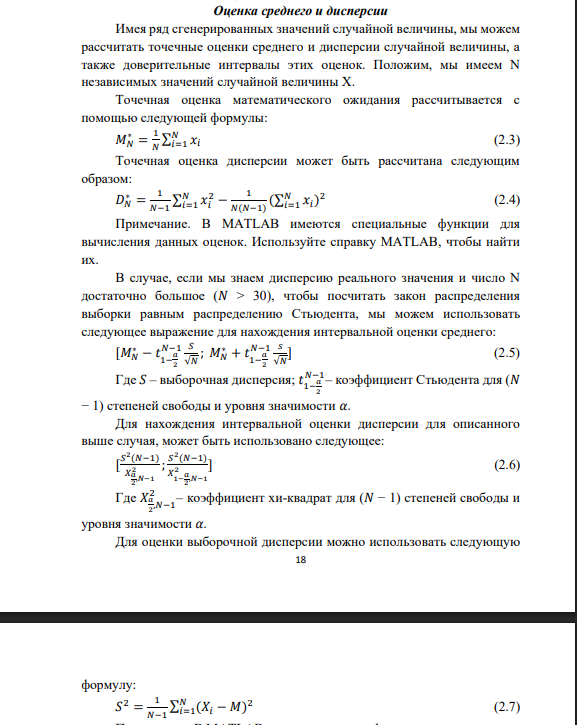
\includegraphics[width=1.0\textwidth]{mean_var_theory.png}
    \caption{Теория для вычисления базовых параметров случайной величины}
\end{figure}

Реализация:\\

\begin{figure}[H]
    \centering
    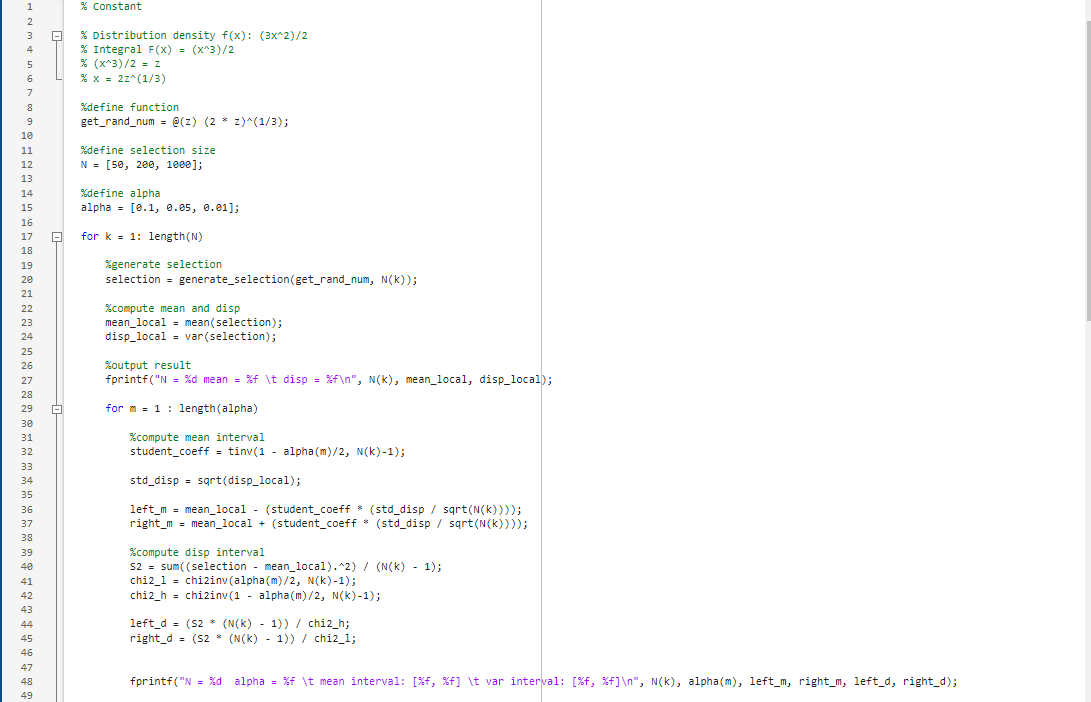
\includegraphics[width=1.0\textwidth]{const_real_1.png}
    \caption{Реализация программы для плотности распределения (часть 1)}
\end{figure}


\begin{figure}[H]
    \centering
    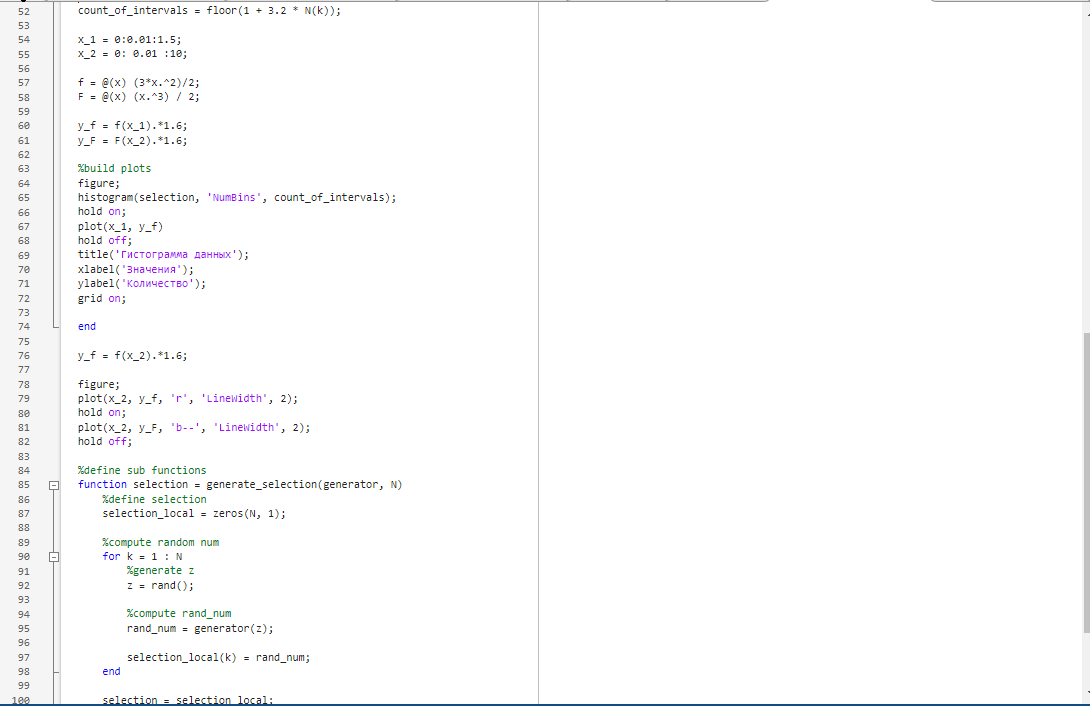
\includegraphics[width=1.0\textwidth]{const_real_2.png}
    \caption{Реализация программы для плотности распределения (часть 2)}
\end{figure}

Результат: \\

\begin{figure}[H]
    \centering
    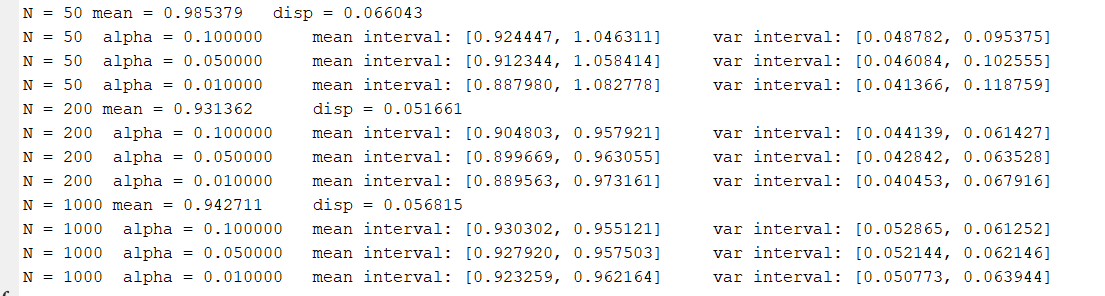
\includegraphics[width=1.0\textwidth]{cmd_res_const.png}
    \caption{Базовые параметры случайной величины для выборок разного объема (N = 50, 200, 1000)}
\end{figure}


\begin{figure}[ht]
    \centering
    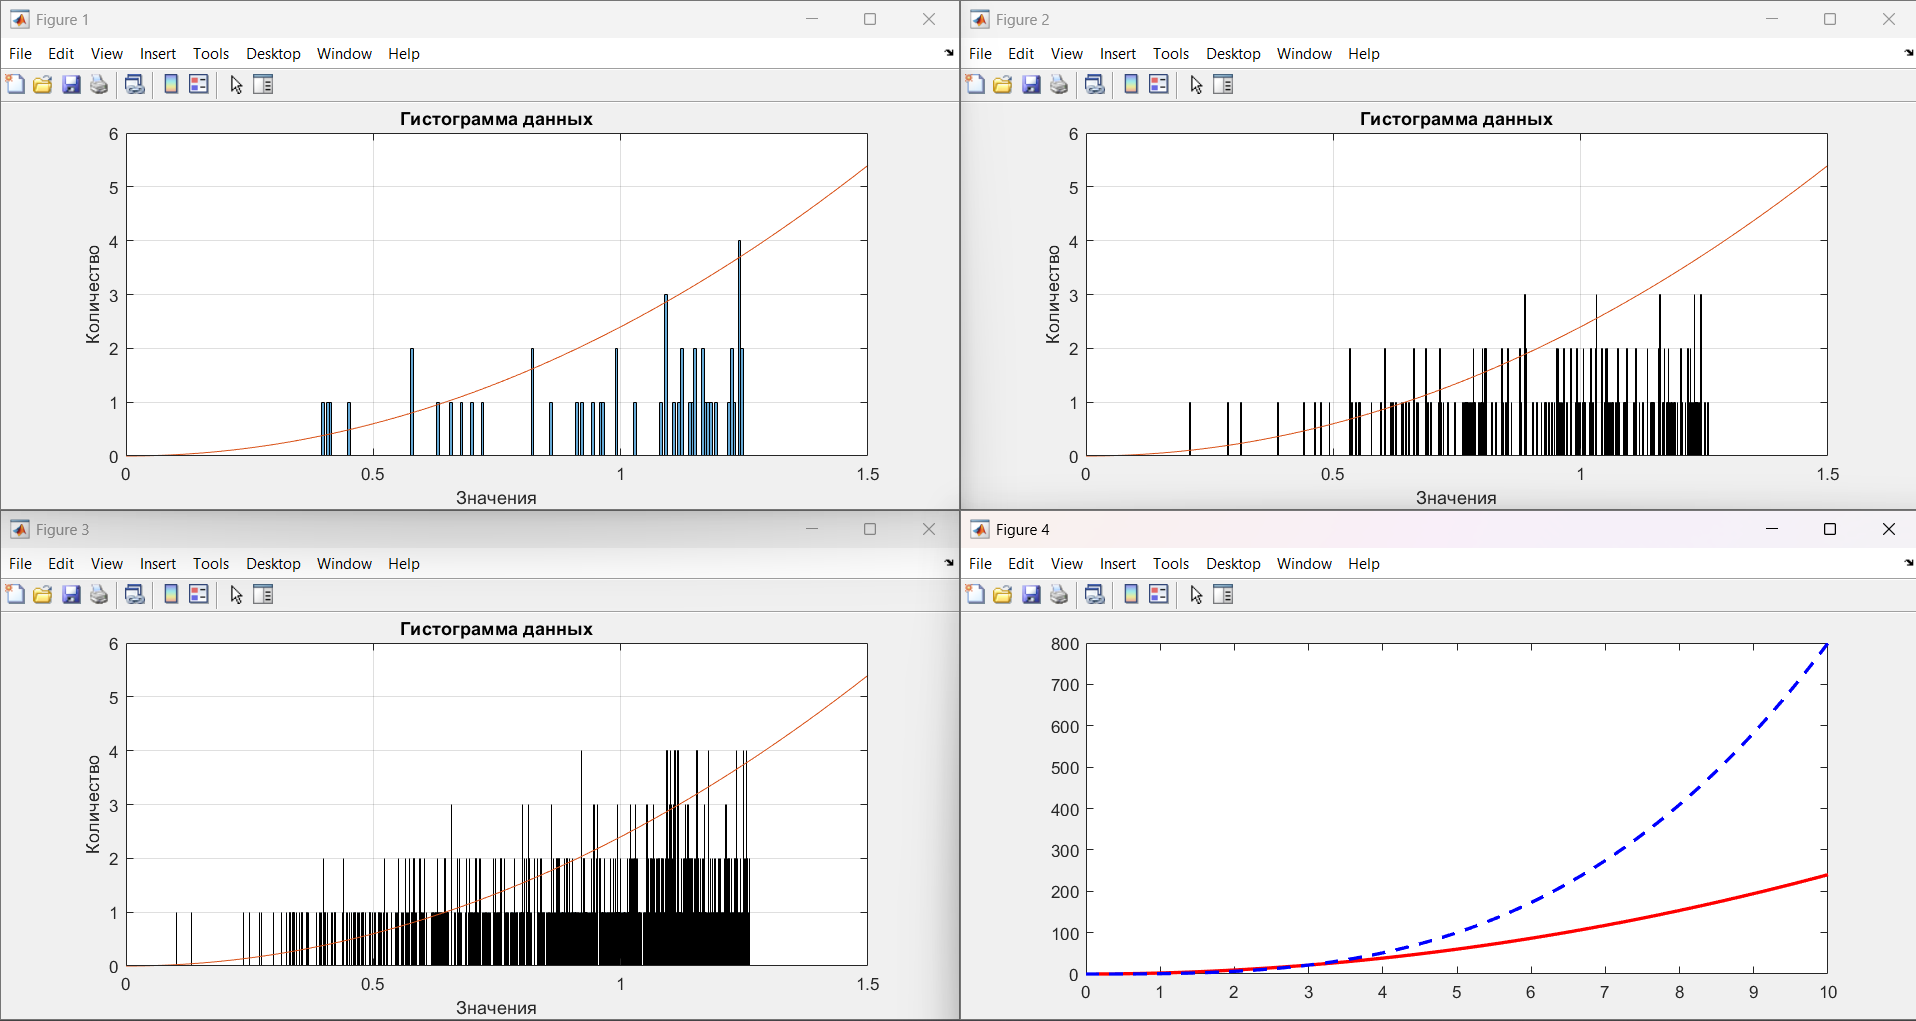
\includegraphics[width=1.0\textwidth]{const_graphs.png}
    \caption{Гистограммы и плотнось распределения для выборок разного объема}
\end{figure}

Последний график визуализирует теоретические плотность распределения и функцию распределения случайной величины.
Гистограмма показывает кол-во чисел, попадающих в определнный промежуток. Кол-во промежутков вычисляются по следующей формуле:

\begin{figure}[ht]
    \centering
    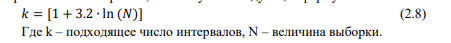
\includegraphics[width=1.0\textwidth]{count_inervals.png}
    \caption{Формула расчета кол-ва интервалов}
\end{figure}



\endinput